x
\documentclass[12pt]{article}
\usepackage{graphicx}
\usepackage{amsmath}
\usepackage{hyperref}
\usepackage{geometry}
\geometry{a4paper, margin=1in}

\title{AI Agents for Autonomous Lunar Navigation and Resource Prospection}
\author{}
\date{}

\begin{document}

\maketitle

\begin{abstract}
The AI Agents for Autonomous Lunar Navigation and Resource Prospection project aims to revolutionize lunar exploration by leveraging advanced artificial intelligence (AI) and robotics. The primary objectives include enhancing autonomous navigation, resource mapping, and data analysis on the lunar surface, reducing reliance on human intervention. AI technologies, such as machine learning, neural networks, and reinforcement learning, will be employed to train agents to operate in the Moon's unique conditions, handling unexpected obstacles and extreme environments. The project will utilize diverse data sources for model training and validation, ensuring robust and reliable AI performance despite challenges like lunar dust and temperature extremes. Human oversight will play a critical role in maintaining transparency, accountability, and ethical decision-making in AI operations. The integration of AI with robotics is expected to significantly enhance lunar exploration capabilities, enabling autonomous habitat construction, in-situ resource utilization, and efficient scientific data processing. The project anticipates a substantial growth in AI deployment in space, aligning with industry projections and supporting future missions with intelligent, autonomous systems.
\end{abstract}

\section{Introduction: Originality of the Research Project}
Spacecraft design is a vast effort, branching out into many fields of science and engineering. The proposed research obtains several important results towards the design of space missions that provide higher utility to the stakeholders, by being more optimized and not bound to the stagnancy of conservative mission design approaches. These improvements are obtained through innovations in three aspects of the mission design: exploring alternative concepts thoroughly and more efficiently.

\begin{figure}[htbp]
    \centering
    \includegraphics[width=0.85\textwidth]{images/introduction:_originality_of_the_research_project_img_1.png}
    \caption{Figure related to Introduction: Originality of the Research Project}
    \label{fig:introduction:_originality_of_the_research_project_1}
\end{figure}

The shift from single-objective to multi-objective problems in mission design is crucial, emphasizing the importance of Pareto-optimal solutions. In this multi-objective setting, the concept of the best design (i.e., the global optimum) is substituted with that of a Pareto front, a collection of non-dominated solutions expressing the trade-offs between different conflicting objectives. Consequently, a set of best possible solutions (Pareto-optimal front) is required to guide engineering decisions.

\section{Hypothesis, Research Objectives, and Envisaged Methodology}
The hypothesis of this research is that AI can significantly enhance lunar exploration capabilities. The research objectives include autonomous navigation, resource mapping, and data analysis on the lunar surface. The methodology involves the use of machine learning, neural networks, and reinforcement learning. Diverse data sources are crucial for model training and validation to ensure robustness and reliability.

\begin{figure}[htbp]
    \centering
    
\includegraphics[width=0.85\textwidth]{images/hypothesis,_research_objectives_and_envisaged_methodology_img_1.png}
    \caption{Figure related to Hypothesis, Research Objectives and Envisaged Methodology}
    \label{fig:hypothesis,_research_objectives_and_envisaged_methodology_1}
\end{figure}

Multi-objective trade-offs are a significant aspect of this research, where solutions must balance between different objectives such as cost and reliability. The Pareto-optimal solutions provide a framework for these trade-offs, ensuring that no objective can be improved without compromising another.

\section{Expected Outcomes / Impact}
The integration of AI with robotics is expected to enhance lunar exploration significantly. This includes autonomous habitat construction and in-situ resource utilization. The efficiency of scientific data processing is anticipated to improve, supporting the growth in AI deployment in space and aligning with industry projections.

\section{Explanations on the Management of Ethical Issues and Data Protection}
Ethical considerations are paramount, including transparency, accountability, and minimizing bias in AI decision-making. Data protection measures such as access management, data version control, and standardization are critical. Human oversight ensures ethical standards and AI reliability.

\begin{figure}[htbp]
    \centering
    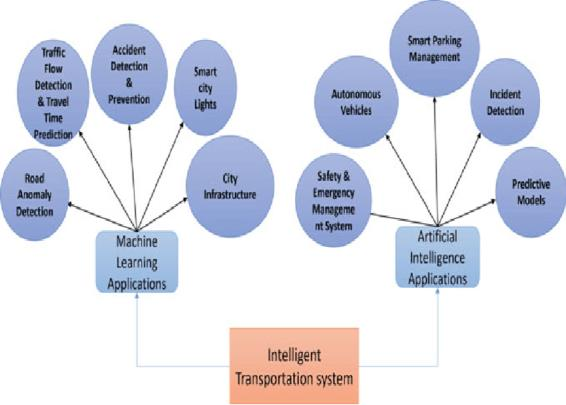
\includegraphics[width=0.85\textwidth]{images/explanations_on_the_management_of_ethical_issues_and_data_protection_img_1.png}
    \caption{Figure related to Explanations on the management of ethical issues and data protection}
    \label{fig:explanations_on_the_management_of_ethical_issues_and_data_protection_1}
\end{figure}

\section{Comment on Resubmission (if applicable)}
Revisions have been made to the methodologies and findings based on feedback from previous submissions. These updates have improved the research's robustness and applicability.

\begin{figure}[htbp]
    \centering
    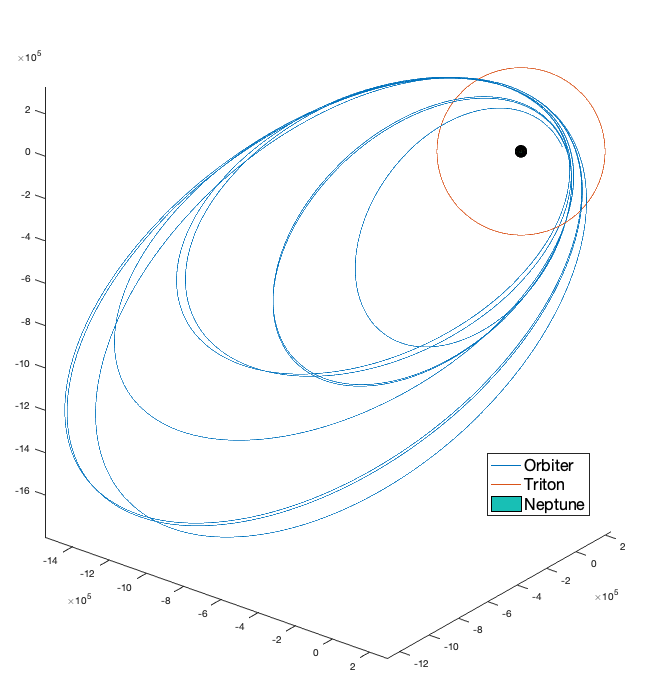
\includegraphics[width=0.85\textwidth]{images/comment_on_resubmission_(if_applicable)_img_1.png}
    \caption{Figure related to Comment on resubmission (if applicable)}
    \label{fig:comment_on_resubmission_(if_applicable)_1}
\end{figure}

\section{Bibliography}
\begin{enumerate}
    \item Eirates), Northrop Grumman Corporation (United States), and the SmartSat Cooperative Research Centre (Australia) for their support of this work through the Grant No. FSU-2022-013, the Collaborative Research Project No. RE-04143, and the Doctoral Research Project No. 2.13s, respectively.
    \item Analysis Once we concluded the study, we transcribed the audio from the sessions and compiled the survey responses.
    \item Relatively inflexible paradigms. Declaration of competing interest The authors declare that they have no known competing financial interests or personal relationships that could have appeared to influence the work reported in this paper.
    \item Can be solved by improving the data used and then the learning method used, rather than hand-crafting the knowledge into the problem.
    \item Across those meetings, though we also encouraged them to break into reflective discussions about the process and tools along the way.
    \item Source DB DB Query Object Graph Fig. 1 Functional diagram of the Prepare step of the AI/ML workflow.
    \item Population. The three genetic operators commonly used are: selection, crossover, mutation.
    \item Proportionate and ordinal methods. Proportionate selection chooses individuals by comparing the fitness values, while ordinal selection selects the individual by comparing the order in which they appear when the population is ranked.
    \item References [61] M. F. M?ller and M. Fodslette, “A scaled conjugate gradient algorithm for fast supervised learning,” Neural Networks, vol. 6, no. 4, pp. 525–533, Jan. 1993.
    \item And their application in other fields of human expertise. In this sense, the research was directed towards medicine and diagnosis.
    \item Applied. The main objective of the selection operator is to pick the fit solutions and eliminate the weak individuals.
    \item Rigorously controlled experiments on human beings (Helmholtz, Wundt, XX century).
    \item Whitehead’s formal analysis of propositional logic and Turing’s theory of computation.
    \item To the reader. We decided to give importance to work published in the last few years, avoiding the historical perspective of older and well-established fundamental works.
    \item Calculus and matrix algebra, the tools of control theory, lend themselves to systems that are describable by sets of variables, whereas AI was founded in part as a way to escape from these perceived limitations.
\end{enumerate}

\end{document}